\chapter{La chaîne de mesure}
\label{chap:measurement-chain}

\begin{figure}[ht]
   \centering
   \vspace{-5mm}
   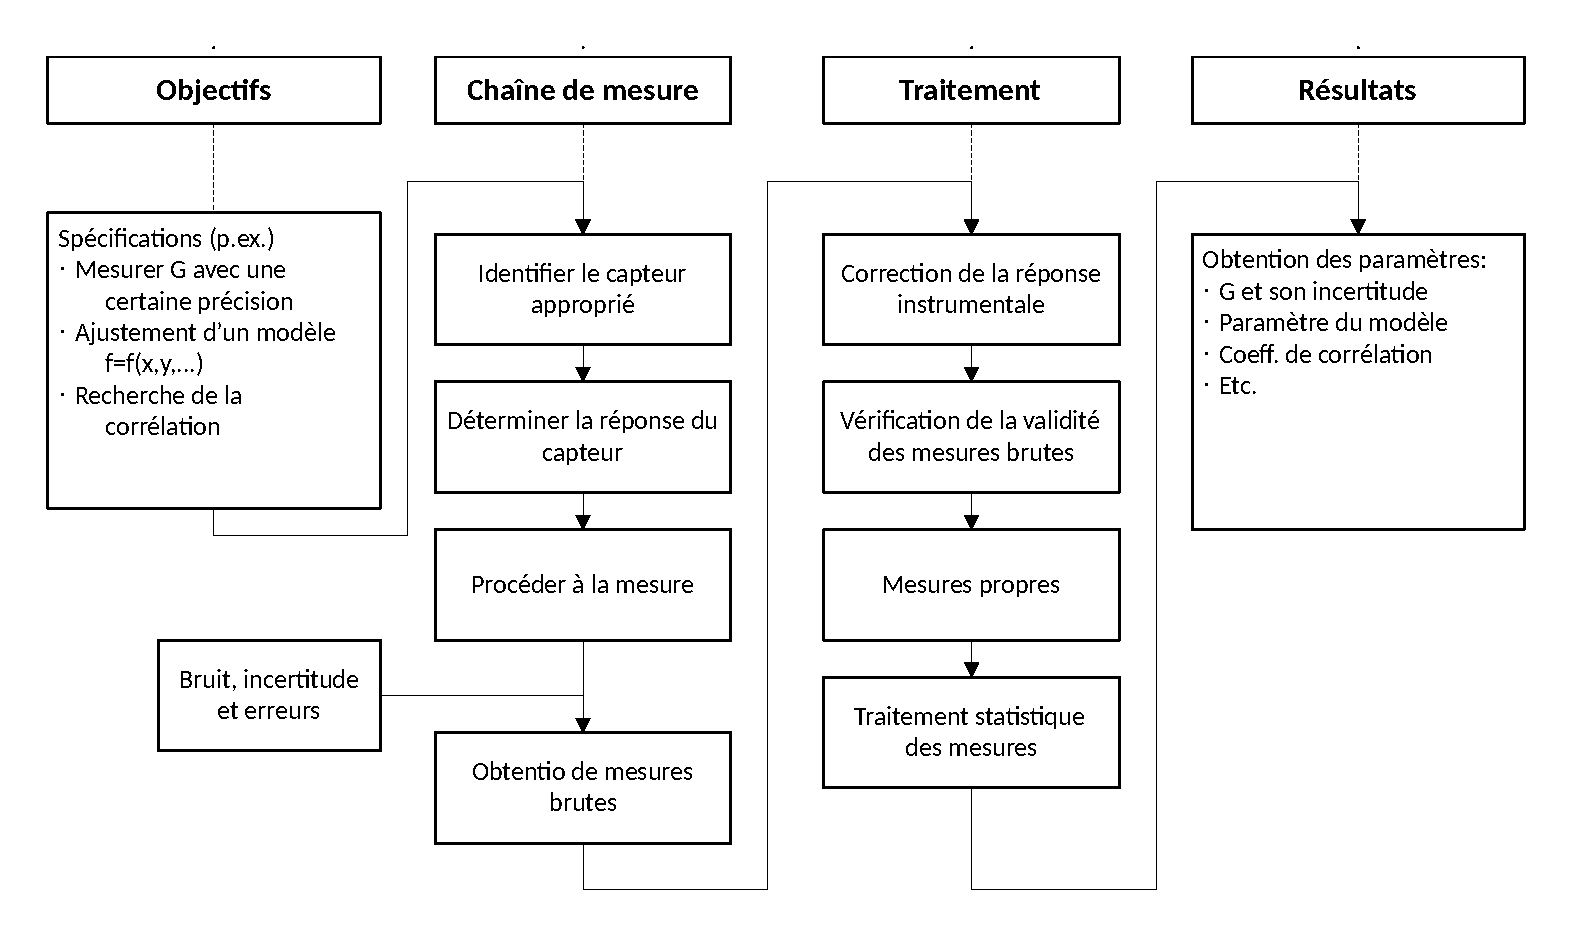
\includegraphics[width=\textwidth]{assets/figures/chaîne-de-mesure-étapes-clés.pdf}
   \caption{Techniques de mesure: les étapes clés.}
   \label{fig:flowChartTechMes_chaine_de_mesure}
\end{figure}

\section{Introduction}

Nous avons vu au chapitre précédent les différents moyens et définitions nécessaires pour que tous les acteurs des techniques de mesure puissent oeuvrer en se comprenant les uns les autres. Reprenant le schéma bloc de la figure \ref{fig:flowChartTechMes_chaine_de_mesure} qui présente les différentes étapes des opérations de mesure, nous nous proposons maintenant d'étudier la chaîne de mesure.

Dans l'instrumentation moderne, on constate pratiquement que chaque équipement ou appareil de mesure comprend un ou plusieurs microprocesseurs. Il convient donc, à l'intérieur du système de mesure de convertir le signal analogique représentant la grandeur que l'on veut mesurer, en une valeur numérique que l'on pourra traiter dans le processeur. Les signaux de sortie d'un capteur sont généralement petits, il est donc nécessaire de les amplifier. D'autre part le capteur doit être placé à un endroit bien précis du processus, à une distance appréciable de l'équipement de mesure (de l'ordre du mètre -- p.e. oscilloscope, à plusieurs centaines de mètres -- pour de grands systèmes).

Il faut donc transmettre l'information entre le capteur et le système de mesure proprement dit. L'information concernant la grandeur à mesurer va ainsi traverser une série d'éléments et d'appareils avant d'apparaître comme résultat de mesure. Cette succession d'appareils ou éléments est appelée une \textbf{chaîne de mesure}.

\begin{definition}
    Une chaîne de mesure est une succession d'appareils et d'éléments assurant la transmission et la transformation de l'information entre le capteur et le résultat de mesure.
\end{definition}

\begin{definition}
    La mesurande $X$ (\emph{measurand}) est la grandeur d'entrée que l'on désire mesurer.
\end{definition}

\begin{figure}[ht]
   \centering
   \vspace{-5mm}
   \includegraphics[width=\textwidth]{assets/figures/chaîne-de-mesure.pdf}
   \caption{Éléments d'une chaîne de mesure. De gauche à droite: le \textbf{capteur}, puis le bloc du \textbf{traitement de signal} (électrique en général), suivi du \textbf{circuit de mesure.}}
   \label{fig:chaine_de_mesure}
\end{figure}
Comme on peut le voir sur la figure \ref{fig:chaine_de_mesure}, une chaîne de mesure comprend toujours au moins trois éléments : le capteur, un circuit de traitement du signal électrique et un élément de mesure.

\begin{itemize}
\item Le capteur  convertit le mesurande en une grandeur électrique brute (caractéristique non linéaire, bruit et perturbations ajoutés à l'information)
\item Le traitement du signal électrique, constitué d'un ou plusieurs éléments, utilise l'information contenue dans la grandeur électrique brute pour obtenir une grandeur électrique épurée, dotée d'un meilleur rapport signal/bruit et d'une exploitabilité facilitée. Ensuite on pourra la manipuler facilement, l'amplifier, la transmettre sur une distance suffisante. Par exemple si la grandeur électrique brute est une résistance, un circuit devra injecter un courant dans la résistance pour obtenir une tension proportionnelle, c'est le conditionneur ; après il faudra probablement soustraire de sa sortie la valeur équivalente au  zéro du mesurande. Dans la plupart des cas le conditionneur et l'amplificateur de transmission sont incorporés dans le même boîtier, désigné comme transmetteur. Ce dernier peut même être monté à l'intérieur de la structure du capteur proprement dit, l'utilisateur ne pouvant alors choisir qu'une ou deux options de grandeur électrique de transmission. À l'autre extrémité du canal de transmission, on trouve un récepteur capable de décoder le signal transmis avant de l'appliquer au circuit de mesure.
\item La mesure  proprement dite consiste à comparer le signal épuré avec l'équivalent de l'unité de mesure,  pour obtenir une valeur numérique de représentation du mesurande (un convertisseur A/D comprend toujours une tension de référence interne représentant l'unité de mesure; dans un appareil analogique, l'unité de mesure est matérialisée: ce sont les marques sur l'écran d'affichage de l'appareil)
\item Un traitement numérique  de la mesure peut encore être ajouté à la chaîne pour améliorer l'élimination du bruit, linéariser le résultat ou combiner les valeurs de plusieurs mesurandes en un résultat de mesure indirecte (par exemple déduire une énergie de la mesure d'un débit et d'une différence de température). Une transmission à distance peut également intervenir à ce niveau, vers un régulateur, un ordinateur central ou une salle de commande.
\end{itemize}
Certains éléments de la chaîne de mesure peuvent être partagés entre plusieurs mesurandes (économie de place, coût de l'installation), mais la conception et l'analyse du système de mesure peut toujours mener à une décomposition en  chaînes de mesure affectées momentanément à chaque mesurande.


\section{Transducteurs: capteurs et actionneurs}

\begin{definition}
    Est qualifié de transducteur (\emph{transducer}) tout élément assurant la liaison entre le monde physique (processus à contrôler, expérience, appareil à vérifier) et l'instrumentation proprement dite. Il convertit la grandeur physique en une grandeur mesurable, ou  à l'inverse, il convertit une grandeur générée par le système de mesure en une grandeur physique permettant d'agir sur le processus.
\end{definition}

\begin{definition}
    Un capteur (\emph{sensor}) est un élément transducteur destiné à la mesure proprement dite : Conversion d'une grandeur physique du processus en une grandeur (généralement électrique) d'entrée du système de mesure. Par exemple un thermocouple est un capteur de température, dont la sortie est une tension électrique dépendant de la température.
\end{definition}

\begin{definition}
    Un actionneur (\emph{actuator}) est un élément transducteur destiné à l'action sur le processus : Conversion d'une grandeur de sortie du système de mesure en une grandeur physique agissant sur le processus. Par exemple une pompe est un actionneur.
\end{definition}

Le capteur est construit pour exploiter une propriété de la matière, décrite par une \textbf{loi physique}, permettant de connaître la correspondance entre la grandeur électrique à la sortie du capteur et la grandeur physique à mesurer. Par exemple, pour mesurer une pression, on peut utiliser la résistance d'un fil et exploiter la loi de la piézorésistivité exprimant la variation de la résistance en fonction de la déformation du fil imposée par la pression. Ainsi à chaque valeur de la résistance correspond une valeur particulière de la pression et la loi physique nous permet de calculer la pression à partir de la mesure de la résistance du capteur. Attention de ne pas confondre avec la piézoélectricité, qui consiste en une génération ou absorption de charges électriques en fonction de la déformation du matériau.

\begin{figure}
   \centering
   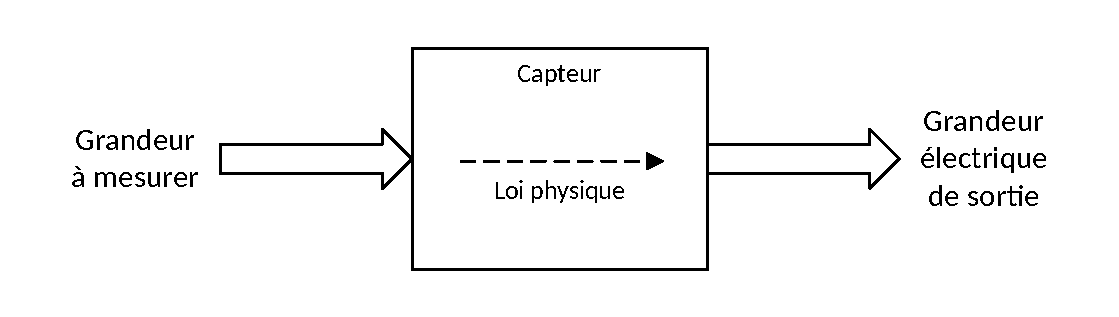
\includegraphics[width=0.96\textwidth]{assets/figures/loi-physique.pdf}
   \caption{Capteur idéal}
   \label{fig:Loi_Physique}
\end{figure}

Malheureusement le capteur étant un élément réel, le comportement de la grandeur de sortie ne peut être décrit par une seule et unique loi physique: Tout irait bien si, dans notre exemple, la déformation du fil n'était due qu'à la pression; en fait des vibrations, ou une modification de la température peuvent également provoquer une légère déformation du fil, donc une variation non désirée de la résistance; plus grave encore, la température provoque directement une variation de la résistance, indépendante de la déformation et décrite par une autre loi physique.
\begin{figure}
   \centering
   \includegraphics[width=0.96\textwidth]{assets/figures/capteur-réel.pdf}
   \caption{Capteur réel}
   \label{fig:Grandeur_Influence}
\end{figure}

Il faut donc bien admettre qu'un capteur n'est jamais idéal, et qu'il doit être représenté par une combinaison de lois physiques, reliant la grandeur de sortie à différentes grandeurs d'entrées. L'une d'entre elles est la grandeur que l'on désire mesurer, appelée le \textbf{mesurande}, les autres sont des \textbf{grandeurs d'influence} car elles modifient la sortie et nous font croire à une variation de la grandeur désirée: le résultat de mesure est influencé par ces grandeurs.

\begin{definition}
Les grandeurs d'influence $Zi$ sont toutes les grandeurs d'entrée non désirées du système, dont l'effet sera de modifier la grandeur de sortie.
\end{definition}

\begin{itemize}
    \item Les grandeurs d'influence les plus courantes sont:
    \item La température -- elle modifie les valeurs des composants électriques (dimensions, résistivité, tension de seuil dans les composants à semi-conducteur, ...)
    \item les tensions d'alimentation - elles modifient la polarisation des éléments, donc leur caractéristique, et indirectement leur température
    \item Le temps -- Les éléments vieillissent et se modifient avec le temps, d'où une dérive lente des caractéristiques.
    \item L'humidité relative -- modifie la constante diélectrique des isolants, provoque des courants de fuite
\end{itemize}

\section{Résolution du problème de mesure}

Dans le processeur du système ou de l'appareil de mesure, on ne dispose que de la sortie numérique $Y$ de la chaîne de mesure. Le problème est donc d'estimer la valeur du mesurande, à partir de la sortie $Y$, et de la connaissance de la caractéristique de la chaîne. Sachant que $Y$ dépend non seulement de $X$, mais aussi des tolérances de fabrication, des grandeurs d'influences, du bruit interne dans les éléments de la chaîne, des perturbations ajoutées par l'environnement, ainsi que de l'effet produit par la présence du capteur sur l'objet mesuré, une solution exacte est impossible.

Il convient donc d'établir un modèle mathématique de la chaîne de mesure, valable dans un certain domaine des conditions d'utilisation, et représentant une approximation de la réponse réelle

\begin{equation}
Y=\mathcal{F}(X)
\end{equation}

L'opération mathématique inverse ne nous donnera qu'une estimation de la valeur du mesurande,

\begin{equation}
X_m=\mathcal{F}^{-1}(Y)
\end{equation}

\begin{definition}
    La vraie valeur $X$ est la valeur du mesurande, que l'on ne connaîtra jamais exactement.
\end{definition}

\begin{definition}
    La valeur mesurée $X_m$ est la valeur indiquée par l'appareil de mesure une estimation de $X$.
\end{definition}

Le fabricant d'un instrument de mesure ne peut spécifier l'incertitude de son appareil que pour un domaine bien défini des grandeurs d'influence, et en l'absence de perturbations externes.

Une fois qu'on a obtenu une estimation $X_m$ du mesurande, il reste à déterminer quelle confiance on peut accorder à ce résultat. C'est là tout le problème de l'analyse des mesures.

\begin{definition}
    La \textbf{validité des mesures} est le degré de confiance que l'on peut accorder au résultat chiffré de la mesure.
\end{definition}

En d'autres termes il s'agit de déterminer si l'on mesure vraiment ce que l'on désire, et d'analyser les causes d'erreurs qui peuvent influencer le résultat. Quelque soit l'équipement utilisé, la méthode d'analyse permettant de répondre à ces questions restera la même, alors que le choix proprement dit de la méthode et des appareils exige une connaissance plus détaillée des principes de mesure de la grandeur concernée.

À titre d'exemple, prenons un capteur de température dans une buse d'injection de PVC (fabrication de pièces injectées), réalisé au moyen d'un thermocouple. Si le montage est parfait, la température indiquée est celle du thermocouple, reste à savoir s'il s'agit bien de la température que l'on désire mesurer : pour éviter l'usure, il faut monter le capteur dans la paroi de la buse d'injection. Quelle est l'influence des échanges thermiques entre la masse à injecter, les parois de la buse et le thermocouple ? De plus le signal électrique fourni par le capteur est de l'ordre de quelques millivolts, et dépend de la température ambiante. L'appareillage tient-il correctement compte de la température ambiante ? Les moteurs utilisés dans l'équipement d'injection ne rayonnent-ils pas suffisamment de champ électrique et magnétique pour induire une tension parasite s'ajoutant au signal du thermocouple ? La validité des mesures dépendra des réponses à toutes ces questions.

L'exemple ci-dessus nous montre qu'en plus de l'incertitude de l'instrumentation l'analyse de la validité des mesures doit tenir compte des interactions du système de mesure avec l'objet que l'on veut mesurer ainsi qu'avec tout son environnement.

L'analyse de la validité des mesures consiste à vérifier l'ordre de grandeur des différentes causes d'erreur:

\begin{itemize}
    \item modèle mathématique (non-conformité, ou non-linéarité)
    \item effet des grandeurs d'influence (modification du comportement de la chaîne)
    \item bruit interne (limite de détection)
    \item perturbations provoquées par l'environnement externe (compatibilité électromagnétique)
    \item effet de charge (échange d'énergie entre l'objet mesuré et la chaîne de mesure)
\end{itemize}

\section{Modèle mathématique}

Du fait des fluctuations possibles de la fonction $\mathcal{F}(X)$, les fabricants se contentent de spécifier une approximation mathématique aussi simple que possible à résoudre. Cette approximation ne sera bien sûr pas valable quelle que soit la valeur du mesurande, mais elle se limite à un intervalle bien précis, appelé \textbf{étendue de mesure}.

\begin{definition}
    L'\textbf{étendue de mesure} est le domaine des valeurs du mesurande dans lequel le modèle mathématique est valable. En d'autres termes c'est le domaine du mesurande pour lequel le fabricant peut garantir l'incertitude de mesure.
\end{definition}

Bien entendu, l'étendue de mesure sera toujours limitée. Au-delà, soit la sortie diverge, soit elle sature. Par exemple sur un simple amplificateur, lorsque la sortie s'approche de la tension d'alimentation, une saturation intervient.

\section{Forme linéaire du modèle de la chaîne de mesure}

C'est la forme mathématique que l'on retrouve dans la grande majorité des cas. En effet, quelque soit la forme de $\mathcal{F}(X)$, pour une étendue de mesure suffisamment faible il est toujours possible de remplacer la courbe $\mathcal{F}(X)$ par un segment de droite. Nous l'écrirons

\begin{equation}
Y = G\cdot X + O
\end{equation}

où le facteur de multiplication $G$ est le \textbf{gain} linéaire de la chaîne de mesure, et $O$ est l'offset, extrapolation de $Y$ en $X=0$.

\section{Forme polynomiale du modèle de la chaîne de mesure}

Lorsque l'étendue de mesure désirée ne permet plus une approximation linéaire, on utilise souvent un polynôme de degré $n$:

\begin{equation}
Y = a_0 + a_1\cdot X + a_2\cdot X^2 + ... + a_n \cdot X^n
\end{equation}

La forme générale de la réponse est donnée par les $n+1$ coefficients $a_0$ à $a_n$. Ceux-ci sont en général imposés par le type de capteur plutôt que par la chaîne de mesure, mais en général, dans la chaîne, au moins un amplificateur permet d'ajuster tant le décalage $a_0$, qu'un gain global, facteur de multiplication des coefficients $a_1$ à $a_n$.

La résolution du problème de mesure implique l'inversion de la fonction, ce qui revient à utiliser un autre polynôme de degré n exprimant X en fonction de Y ; c'est souvent ce polynôme qui est recherché par régression mathématique:

\begin{equation}
X_m = c_0 + c_1\cdot Y + c_2\cdot Y^2 + .... + c_n\cdot Y^n
\end{equation}

\paragraph{Exemple de modèle quadratique: capteur de débit à déprimogène}

En plaçant un obstacle dans un fluide dont on désire mesurer le débit (constitué d'un diaphragme, d'un tube Venturi, Pitot ou autre), on provoque localement une différence de pression proportionnelle au carré de la vitesse du fluide à mesurer (loi de Bernoulli, $\Delta p=a_2v^2$). En mesurant la perte de pression, on peut donc mesurer la vitesse du fluide, et partant, son débit, si le fluide est pare exemple confiné dans un tube. En pratique, cependant, $a_2$ ne peut être considéré comme constant que pour une étendue de mesure assez limitée: débits variant dans un rapport 1 à 3 seulement, car d'autres lois interviennent (détente adiabatique, frottements, turbulence, etc.)

\paragraph{Exemple de modèle polynomial à degré élevé: mesure de température par thermocouple}

Un thermocouple (TC) est la combinaison de 2 conducteurs de matériau différents A et B. La jonction chaude (ou soudure chaude, dont on veut mesurer la température) est le point de contact entre A et B. Les jonctions froides (ou soudures froides) sont les liaisons de A et B avec le circuit de mesure (fils de cuivre). Elles sont en principe à la température ambiante.

La tension que le TC produit est uniquement fonction des températures des jonctions chaudes et froides, et est de l'ordre de 5 à 50 $\mu$V/$\degree C$ selon les types de matériaux. Les fabricants fournissent des tables indiquant degré par degré la tension produite lorsque les jonctions froides sont à 0$\degree$C. Puisque ces dernières sont, en pratique, à la température ambiante, il est indispensable de prévoir une correction.

% TODO: Why is this code commented out?
%La théorie de la thermoélectricité nous indique que la tension indiquée dans les tables est égale à la somme de la tension produite UTC lorsque les jonctions froides sont à une température différente de zéro et de la tension indiquée dans les tables des fabricants à la température des jonctions froides Utable(Tfr):
%\begin{equation}
%\mathcal{U}_{table}(T_{ch}) = \mathcal{U}_{TC} + \mathcal{U}_{table}(T_{fr})
%\end{equation}
%Le circuit de mesure doit donc non seulement mesurer UTC, mais également la température des jonctions froides $T_{fr}$ (au moyen d'un $2^e$ capteur). La résolution du problème de mesure consiste d'une part à retrouver $U_{table}(T_{fr}$) pour permettre le calcul de $U_{table}(T_{ch}$), puis à calculer $T_ch$ à partir de $U_{table}(T_{ch})$.

Pour de grands domaines de températures, cette opération exige d'utiliser, pour le modèle, un polynôme du 9e degré.

% TODO: Why is this code commented out?
%, alors que pour la compensation de jonction froide le domaine 0 à 50  $\degree$ C est suffisant et peut être approché par un polynôme du $2^e$ degré seulement.

\section{Loi physique du capteur}

Enfin, plus rarement, le modèle découle directement de la loi physique exploitée dans le capteur, si besoin corrigée et complétée par des termes de type expérimental.

\paragraph{Exemple : Mesure de température par thermistance}

Une thermistance est une résistance en mode semi-conducteur, dont la valeur varie avec la température, selon

\begin{equation}
R(T) = R_{25}\exp{\left[b\left(\frac{1}{T}-\frac{1}{298}\right)\right]}
\end{equation}

où $T$ est en kelvin, $R_{25}$ est la résistance à 25$\degree$C, c.-à-d. 298$\degree$K, et $b$ un coefficient (en kelvin) caractéristique du semi-conducteur. En inversant la fonction, on trouve:

\begin{equation}
\frac{1}{T} = \frac{1}{b}\ln{\left(\frac{R}{R_{25}}\right)}+\frac{1}{298} = A + B\,\ln{R}
\end{equation}

L'expérience montre cependant que le coefficient $b$ ne peut être considéré comme constant que dans un faible domaine de température (15 à 25$\degree$C), par conséquent l'équation ci-dessus a été complétée (à la manière polynomiale) suivant

\begin{equation}
\frac{1}{T} = A + B \ln{R} + C \ln^3{R}
\end{equation}

Cette expression est alors valable dans un domaine de 100 à 150$\degree$C avec une incertitude de l'ordre de 0.01$\degree$ C.

\section{Erreurs de non-conformité ou de non-linéarité}

À l'intérieur du domaine de mesure, le modèle mathématique ne fait que s'approcher et lisser la réponse réelle. Ceci conduit à des erreurs que l'on appelle de manière générale erreurs de non-conformité, ou de non-linéarité dans le cas d'un modèle linéaire. Ces notions seront traitées dans le chapitre 4.

\section{Bruit interne}

La conduction électrique se faisant par déplacement de charges électriques élémentaires, le signal de sortie ne peut être rigoureusement constant même si les conditions d'utilisation ne changent pas. On constate l'addition d'un petit signal aléatoire à l'information souhaitée : c'est le bruit interne d'agitation thermique dans les résistances, ou le bruit de grenaille typique dans les jonctions de semi-conducteurs. Si ces bruits sont généralement négligeables, ils représentent cependant la limite absolue de détection du circuit: en effet, pour pouvoir distinguer une variation du signal, il faut que celle-ci soit significativement plus grande que la fluctuation aléatoire du bruit interne du système.

\section{Grandeurs d'influence}

Comme déjà indiqué, la grandeur de sortie d'un capteur dépend non seulement du mesurande, mais également d'autres grandeurs physiques, comme la température par exemple. Ces autres grandeurs physiques sont appelées grandeurs d'influence.

La spécification d'incertitude, donnée par le fabricant, tient compte du bruit interne ainsi que des grandeurs d'influences, dans un domaine particulier, qu'il se doit d'indiquer dans les spécifications, par exemple $23\pm5^\circ$C, alimentation 220 V$\pm$10\%.

Le rôle de l'opérateur est donc d'abord de vérifier que les grandeurs d'influence sont bien à l'intérieur du domaine prévu par le constructeur, au moment où l'on effectue les mesures. Ensuite seulement, il pourra utiliser l'incertitude comme critère de validité. Lorsque les grandeurs d'influence sortent des domaines d'utilisation prévus, il convient de tenir compte des coefficients d'influence, ou de calibrer l'instrumentation.

\section{Effet de charge}

L'interaction entre l'objet à mesurer et le système de mesure exige un transfert d'énergie, si petit soit-il. La présence du capteur, et du système de mesure va donc un tant soit peu modifier l'état du processus que l'on cherche à observer. Il devient donc impossible de connaître l'état qu'aurait le processus en l'absence du système de mesure, mais en choisissant correctement le capteur et le système, on peut minimiser ces effets, et s'approcher de la \textless\textless\ vraie\ \textgreater\textgreater valeur qu'aurait le processus \textless\textless\ à vide\ \textgreater\textgreater.

Le transfert d'énergie, n'est pas la seule cause d'effet de charge: pour pouvoir insérer le capteur à l'endroit de la mesure, il faut généralement modifier la structure de l'objet, donc en modifier le comportement. La difficulté est alors de choisir un capteur et un lieu de mesure permettant d'éviter trop de modifications du comportement du processus, tout en maintenant la possibilité d'obtenir des mesures significatives.

\begin{definition}
L'effet de charge (\emph{loading effect}) est la modification de l'état du processus et du système de mesure dû aux sorties non désirées du transducteur (échange d'énergie) ou au changement de structure  du processus imposé par la présence du transducteur.
\end{definition}

\paragraph{Exemples}

\begin{enumerate}
    \item Un voltmètre a toujours une résistance interne $R_v$. La mesure de la tension de charge $U_b$ d'une batterie de résistance interne $R_i$ s'accompagne du passage d'un courant $i = U_b/(R_i+R_v)$. La puissance transférée au voltmètre est donc $P=U_v\cdot i$. L'effet de charge se traduit donc par le fait que le voltmètre ne mesure pas exactement $U_b$, mais

    \begin{equation}
    U_v=U_b\cdot\frac{R_v}{R_v+R_i}
    \end{equation}

    \item Pour mesurer la résistance d'une jauge de contrainte, il faut faire passer un courant dans le fil. Ce courant provoque un échauffement du capteur, qui se transmet au support et conduit à une modification de la grandeur d'influence (la température), donc de la grandeur de sortie. Il y a  effet de charge par échange d'énergie. De plus, le fait de coller la jauge sur son support modifie la constante d'élasticité locale. Pour une même contrainte, la déformation sera légèrement différente: c'est un 2e effet de charge dû à une modification de structure du processus.
    \item Pour mesurer la vitesse des gaz à la sortie d'une tuyère, il faut placer une sonde, dans le flux de gaz. Aussi petite que soit la sonde, elle va modifier les lignes de flux. Il y a effet de charge par modification structurelle.
\end{enumerate}

L'effet de charge se traduit par une erreur systématique (= elle se produit toujours dans le même sens: addition d'une petite constante ou multiplication de la valeur mesurée par un facteur proche de l'unité). C'est donc lors de la conception du système de mesure que l'opérateur doit analyser cet effet, et sélectionner une instrumentation adaptée à l'objet mesuré. À noter que puisque l'erreur due à l'effet de charge est systématique, il est possible de la corriger, ce qui est un avantage par rapport aux erreurs de type aléatoires, imprédictibles par nature.

\section{Perturbations}

Le fait que les équipements de mesure et de contrôle sont placés dans un environnement naturel les soumet à des perturbations : rayonnements cosmiques, éclairs dans un orage, bruit intrinsèque dans la matière même des éléments. De plus l'activité humaine est également source de perturbations : émission radio et TV, communications haute fréquence, champs électromagnétiques des lignes de distribution d'énergie, des moteurs et générateurs, étincelles d'allumage des moteurs à combustion, etc. Dans un appareillage électrique, ces perturbations sont couplées par les champs électromagnétiques dans les circuits, ce qui se traduit par une tension ou un courant perturbateur s'ajoutant au signal sur la grandeur de sortie.

L'appareillage doit répondre à des normes de compatibilité électrique, assurant qu'il n'est pas perturbé par des champs externes, et qu'il n'émet pas trop de perturbations. Par ailleurs le câblage entre appareils peut fort bien fonctionner comme antenne, et introduire des perturbations dans le système de mesure.

Il existe des méthodes pour se protéger contre de telles perturbations, essentiellement par le choix du câblage, du type d'amplificateur, et des méthodes de transmission du signal. Lors de l'analyse de validité, il convient de détecter la présence et l'ordre de grandeur des perturbations. Ceci implique une analyse du signal de sortie, soit sous la forme temporelle, mais le plus souvent dans le domaine fréquentiel (détection d'une composante alternative non liée au mesurande).

\section{Systèmes d'acquisition de données}

\begin{definition}
    Le \textbf{système d'acquisition de données} est l'ensemble d'appareils interconnectés de manière à permettre l'obtention automatique d'une série de mesure sur un objet. Ce dernier peut aller d'un simple circuit intégré à une chaîne de fabrication complète.
\end{definition}

L'analyse et le choix des caractéristiques du système de mesure étant fortement liés à l'application, il est clair qu'il n'est pas possible d'énoncer des règles universelles. L'objectif de ce paragraphe est cependant de donner une vision générale de ces systèmes et de leurs composants. Le choix d'une réalisation doit être le résultat d'un travail de synthèse entre les connaissances des moyens de mesure, des structures possibles et des éléments disponibles.

\begin{figure}[h]
\centering
\includegraphics[width=0.9\textwidth]{assets/figures/acquisition-de-données.pdf}
\caption{Système typique d'acquisition de données}
\label{fig:SystemeTypiquedAcquisitionDeDonnees}
\end{figure}

Tout système d'acquisition comprend au moins une chaîne de mesure. Dès que l'on est en présence de plusieurs chaînes se pose la question d'une économie de matériel en exploitant un multiplexage, soit sous forme analogique (sortie des conditionneurs ou transmetteurs connecter successivement à un seul convertisseur A/D), soit sous forme numérique (les convertisseurs sont reliés à l'ordinateur au travers d'un bus numérique).

Dans la majorité des cas, il faut pouvoir agir sur l'objet mesuré au moyen de chaînes d'action. L'action recherchée peut être de type tout ou rien (arrêt d'urgence, enclenchement - déclenchement d'une pompe ou d'un chauffage...) ou de type analogique (envoi d'un stimulus, commande d'une vanne proportionnelle, de la vitesse d'un moteur ...). Dans le premier cas, un signal logique de sortie de l'ordinateur commande un relais permettant d'appliquer ou non une puissance fixe sur l'actionneur. Dans le second cas, la chaîne d'action comprend un convertisseur digital - analogique (D/A) qui commande l'actionneur au travers d'amplificateurs de puissance.

Le coeur du système est son ordinateur ou processeur, chargé de commander la séquence de travail, d'effectuer les calculs nécessaires au traitement numérique, d'assurer le sauvetage et la transmission des données ainsi que de la communication avec l'opérateur du système. Selon le type d'application, on peut se contenter d'un simple microcontrôleur, exploiter un processeur de calcul numérique (DSP) ou devoir exploiter un ordinateur haut de gamme.

\begin{figure}[ht]
    \centering
	\includegraphics[width=0.9\textwidth]{assets/figures/entrées-analogiques.pdf}
	\caption{Carte universelle d'acquisition: entrées analogiques.}
	\label{fig:Analog_Frontend}
\end{figure}

\begin{figure}[ht]
    \centering
	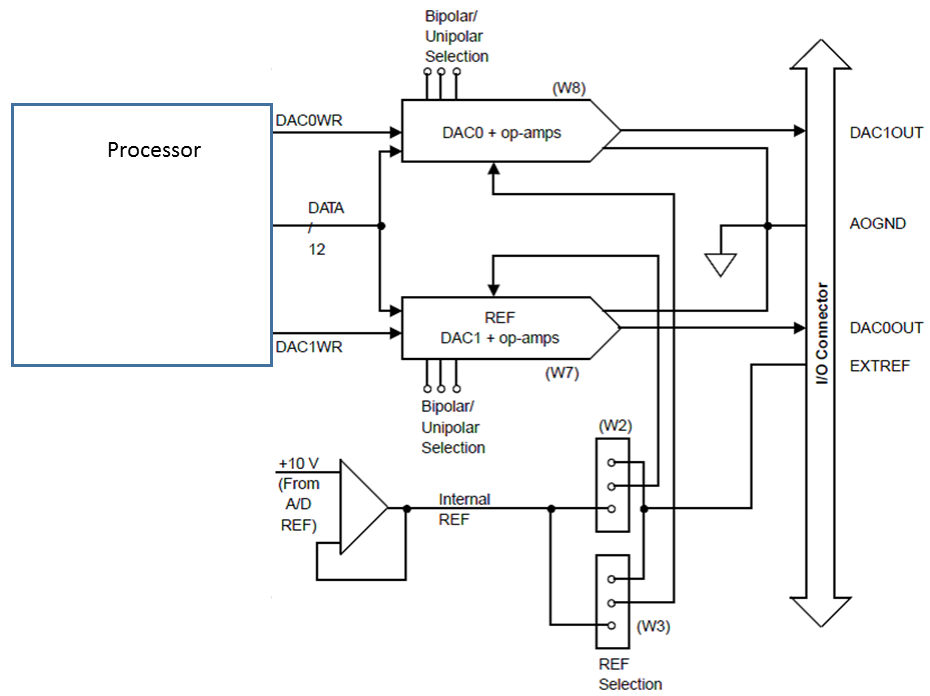
\includegraphics[width=0.9\textwidth]{assets/figures/2_9b_Sorties_analogiques.PNG}
	\caption{Carte universelle d'acquisition: sorties analogiques.}
	\label{fig:Sorties_analogiques}
\end{figure}

\section{Architectures}

Les cartes universelles d'acquisition permettent de réaliser à bon marché des applications d'acquisition et de contrôle de processus. Il ne faut pas oublier cependant que leur résolution et leur précision sont limitées, qu'elles sont sujettes à passablement de bruit (terre de l'ordinateur largement perturbée par les transitoires de la logique rapide) et que les fréquences d'échantillonnage sont limitées tant par le nombre de canaux à mesurer que par la nécessité de les commander directement par le processeur.

Les figures ~\ref{fig:Analog_Frontend} et ~\ref{fig:Sorties_analogiques} présentent une architecture de carte d'acquisition universelle. On constate que l'entrée analogique est formée de 2 multiplexeurs et non d'un seul. Cela permet d'effectuer des mesures différentielles, dans le but d'éliminer les perturbations communes aux deux fils de connexion, à savoir le signal et sa référence si la liaison est asymétrique, ou le signal positif et le signal négatif si la transmission est différentielle. On notera que sur chacun des cas d'entrée ou de sortie, une référence de tension est présente. Sa précision et sa stabilité sont essentielles pour garantir la qualité des mesures.

\section{Modes du multiplexeur}

Trois modes de fonctionnement du multiplexeur analogique sont à disposition:

\begin{itemize}
    \item SE - Asymétrique: Fig.~\ref{fig:Mesure_asymetrique}. Le multiplexeur relie l'une des 16 bornes d'entrée (Ain0 à Ain15) à l'entrée \textless\textless\ hi \ \textgreater\textgreater du PGA, alors que l'entrée \textless\textless\ lo \ \textgreater\textgreater est mise à la masse (gnd) de la carte. On mesure ainsi le potentiel de la borne correspondante par rapport  à la carte. Cette méthode est donc dangereuse, si les sources de signal sont référées à la masse locale : le bruit au niveau de la masse du pc s'ajoute aux signaux mesurés. À n'utiliser que pour des sources de signal flottantes dont on pourra connecter la borne de référence à la masse de la carte!
    \item RSE - pseudo-différentiel ou asymétrique à référence externe : Fig.~\ref{fig:Mesure_Pseudo_differentielle}. le multiplexeur fonctionne de la même manière, mais la borne \textless\textless\ lo \ \textgreater\textgreater du PGA est reliée à la borne \textless\textless\ Aisense \ \textgreater\textgreater du connecteur externe. Il faut alors relier cette borne à la référence zéro (généralement la masse) de l'objet à mesurer. On élimine ainsi les problèmes de bruit au niveau de la masse du PC. Cependant toutes les sources de signal doivent être reliées à ce même point commun \textless\textless\ Aisense \ \textgreater\textgreater.
    \item Diff - Vrai différentiel : Fig.~\ref{fig:Mesure_differentielle}. le multiplexeur est séparé en deux parties travaillant simultanément : la partie A relie le canal i (Ain0 à Ain7) à la borne \textless\textless\ hi \ \textgreater\textgreater, pendant que la partie B relie la borne correspondante i+8 (Ain8 à Ain15) à la borne \textless\textless\ lo \ \textgreater\textgreater. On mesure alors vraiment la différence de potentiel entre un couple de bornes (Ain0 et Ain8, Ain1 et Ain9 ...), mais on ne dispose plus que de 8 canaux. La seule exigence à respecter est que le mode commun reste dans le domaine supporté par le PGA, soit que chacune des bornes reste dans le domaine de $\pm$ 11V par rapport à A-gnd (masse de la carte).
\end{itemize}

\begin{figure}[h]
    \centering
	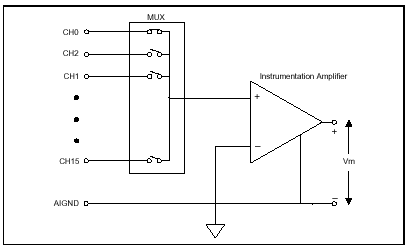
\includegraphics[width=10cm]{assets/figures/2_10_Mesure_asymetrique.PNG}
	\caption{Mesure asymétrique (SE = Single Ended).}
    \label{fig:Mesure_asymetrique}
\end{figure}

\begin{figure}[h]
    \centering
	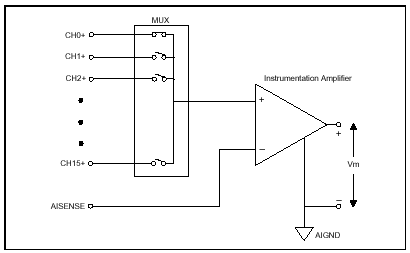
\includegraphics[width=10cm]{assets/figures/2_11_Mesure_Pseudo_differentielle.PNG}
	\caption{Mesure Pseudo-différentielle ou Asymétrique référencée (RSE = Referenced Single Ended).}
	\label{fig:Mesure_Pseudo_differentielle}
    \centering
	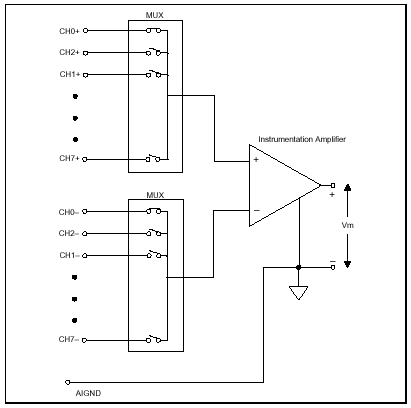
\includegraphics[width=10cm]{assets/figures/2_12_Mesure_differentielle.PNG}
	\caption{Mesure différentielle.}
	\label{fig:Mesure_differentielle}
\end{figure}

\section{Sources flottantes et courants de polarisation}

Lorsqu'on mesure une source flottante, il faut prévoir un chemin de retour vers A-gnd pour les courants de polarisation du PGA (mode RSE et Diff). L'absence d'un tel chemin galvanique provoquerait la saturation du PGA. Ces courants sont inférieurs à 200 pA. Une résistance de l'ordre de 100 kOhms contre A-gnd, suffit, mais afin de ne pas dégrader le taux de réjection du mode commun, il est préférable de connecter une résistance sur chacune des deux entrées (hi et lo). Le dimensionnement de ces résistances se fait en fonction du mode commun : ce montage ajoute un mode commun de (200 pA*100kOhms) = 20 uV généralement négligeables. On voit qu'on pourrait sans autre fortement augmenter la valeur des résistances.

\section{Conditionnement des signaux}

Bien que le fait de disposer d'un PGA permette un grand choix des gammes de mesures (100mV à 10V en unipolaire et +/-50mV à +/-10V en bipolaire), la plupart des applications exigent d'utiliser des circuits de conditionnement  (capteur, atténuateur, amplificateur, shunt ...) avant de relier les signaux à la carte. Le pilote de la carte est généralement capable de tenir compte automatiquement du gain du PGA. Il peut ainsi fournir les résultats des conversions selon deux options:

\begin{itemize}
    \item en V au niveau du connecteur d'entrée (nombre réel).
    \item ou directement le code de conversion sous forme d'un nombre entier (+/-2048).
\end{itemize}

C'est à l'utilisateur de tenir compte des caractéristiques de conditionnement pour calculer l'équivalent de la grandeur mesurée en unités physiques (degrés Celsius, Bar, Kg ...)

\section{Les différents types de signaux}

Un système de mesure transforme une \textbf{entrée}, en règle générale une grandeur physique, en un signal de \textbf{sortie}. Différents types de signaux sont transmis entre les capteurs, les conditionneurs et la sortie du système.

On peut classifier les signaux en trois catégories selon leur représentation temporelle et les valeurs prises par la quantité mesurée (fig.~\ref{fig:typsign1}):

\begin{description}
    \item[Un signal continu] est défini pour toutes les valeurs du temps et peut prendre n'importe quelle valeur en amplitude,
    \item[Un signal discret] est en général un signal continu qui est mesuré à certains instants seulement, mais il peut aussi s'agir d'un signal naturellement discontinu, tel que le nombre de photons reçus par un détecteur pendant une certaine durée de temps, un nombre de véhicules par tranche d'heure sur une route, etc.
    \item[Un signal numérique] est un signal discret quantifié sur un certain nombre de niveaux (généralement des puissances de 2) et qui ne peut prendre qu'un ensemble discret de valeurs, par exemple la numérisation d'un signal électrique de -10 à +10 V sur 8 bits non signés, de 0 à 255.
\end{description}

\begin{figure}[h]
   \centering
   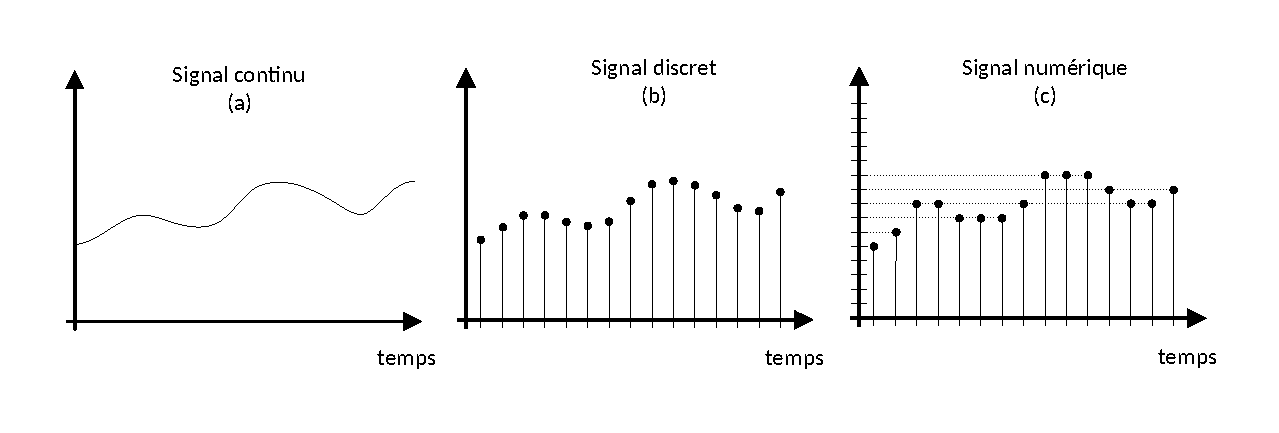
\includegraphics[width=13cm]{assets/figures/types-de-signaux.pdf}
   \caption{Les trois types de signaux les plus fréquents.}\vspace{5mm}
   \label{fig:typsign1}
   \centering
   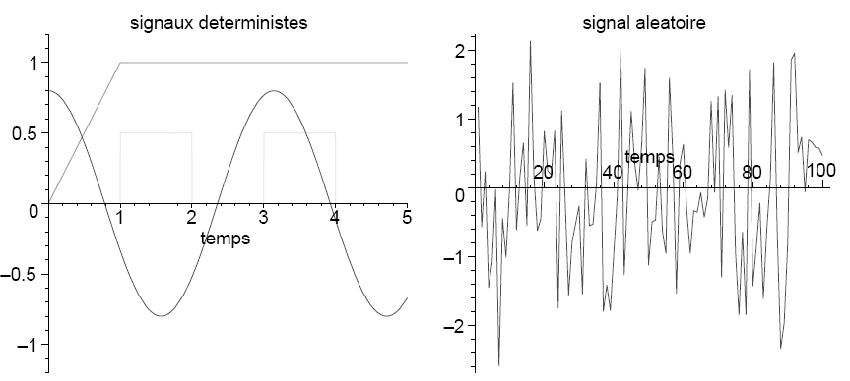
\includegraphics[width=13cm]{assets/figures/sigda.pdf}
   \caption{Signaux déterministes et aléatoires.}
   \label{fig:sigda1}
\end{figure}
En fonction du phénomène physique qu'ils représentent, il faut aussi distinguer les signaux \textbf{déterministes}, c'est-à-dire les signaux pour lesquels les valeurs futures peuvent être prédites, et les signaux \textbf{aléatoires} qui ne sont pas prédictibles et qui nécessitent un traitement spécifique (fig.~\ref{fig:sigda1}).

\pagebreak

\section{Exercices}

\subsection{Exercice: Résistances de polarisation}
La carte d'acquisition MIO16 du labo est spécifiée avec une impédance d'entrée de \SI{100}{\giga\ohm} en parallèle avec 50 pF. Le courant de polarisation d'entrée est de \SI{200}{\pico\ampere}, et le domaine des tensions d'entrée (signal + mode commun) est de \SI{\pm11}{\volt}.

Dimensionner les résistances de polarisation à brancher entre les entrées et la terre A-Gnd de la carte, pour des sources flottantes, dans le cas d'une gamme de mesure de \SI{\pm50}{\milli\volt}, et dans le cas d'une gamme de mesure de \SI{\pm5}{\volt}, en mode différentiel.

\subsection{Exercice: Fréquence de scrutation}
La carte d'acquisition MIO16 du labo est spécifiée avec une impédance d'entrée de \SI{100}{\giga\ohm} en parallèle avec 50 pF. Le convertisseur est un 12 bits - 100 kéch/s. On l'utilise pour mesurer 4 canaux dont les impédances de sortie sont de \SI{5}{\kilo\ohm}. Déterminer s'il faut changer la fréquence de scrutation (critère : établissement à 1 LSB), et quelle est la fréquence maximum d'échantillonnage que l'on pourra obtenir.

\subsection{Exercice: Multiplexage et déphasage}
A l'aide d'une carte 250 kéch/s, on mesure 5 canaux. Calculer quel est le déphasage maximum entre les canaux introduit artificiellement par le multiplexage, en fonction de la fréquence des signaux, ainsi qu'à \SI{1}{\kilo\hertz} et à \SI{10}{\kilo\hertz}.